\documentclass{article}

\usepackage{amsmath, amssymb} % Math formatting and symbols
\usepackage{graphicx} % Insert graphics
\usepackage{wrapfig} % Allow text to wrap around images
\usepackage[cm]{fullpage} % Smaller margins and header/footer
\usepackage{enumitem} % Allow for widest tag in enumerate

\renewcommand*\descriptionlabel[1]{\hspace\leftmargin$#1$}

\newenvironment{adescription}[1]
{\begin{list}{}%
		{\renewcommand\makelabel[1]{##1\hfill}%
			\settowidth\labelwidth{\makelabel{#1}}%
			\setlength\leftmargin{\labelwidth}
			\addtolength\leftmargin{\labelsep}}}
	{\end{list}}

\newcommand{\bd}{\textbf}

\title{Rectangular Coordinates}
\author{}
\date{}

\begin{document}
	
	\maketitle{}
	
		\section{The Distance Formula}
			This distance formula is used to find the \bd{euclidean distance} between two points on the \bd{Cartesian plane}. The distance formula has a strong connection to the Pythagorean theorem.
			\begin{equation}\label{pyt}
				c^2 = b^2 + a^2
			\end{equation}
			The distance formula is essentially the Pythagorean theorem (\ref{pyt}) after replacing the $a$ and $b$ values with \emph{change in x} and \emph{change in y}.
			
			\begin{wrapfigure}{r}{0.28\textwidth}
				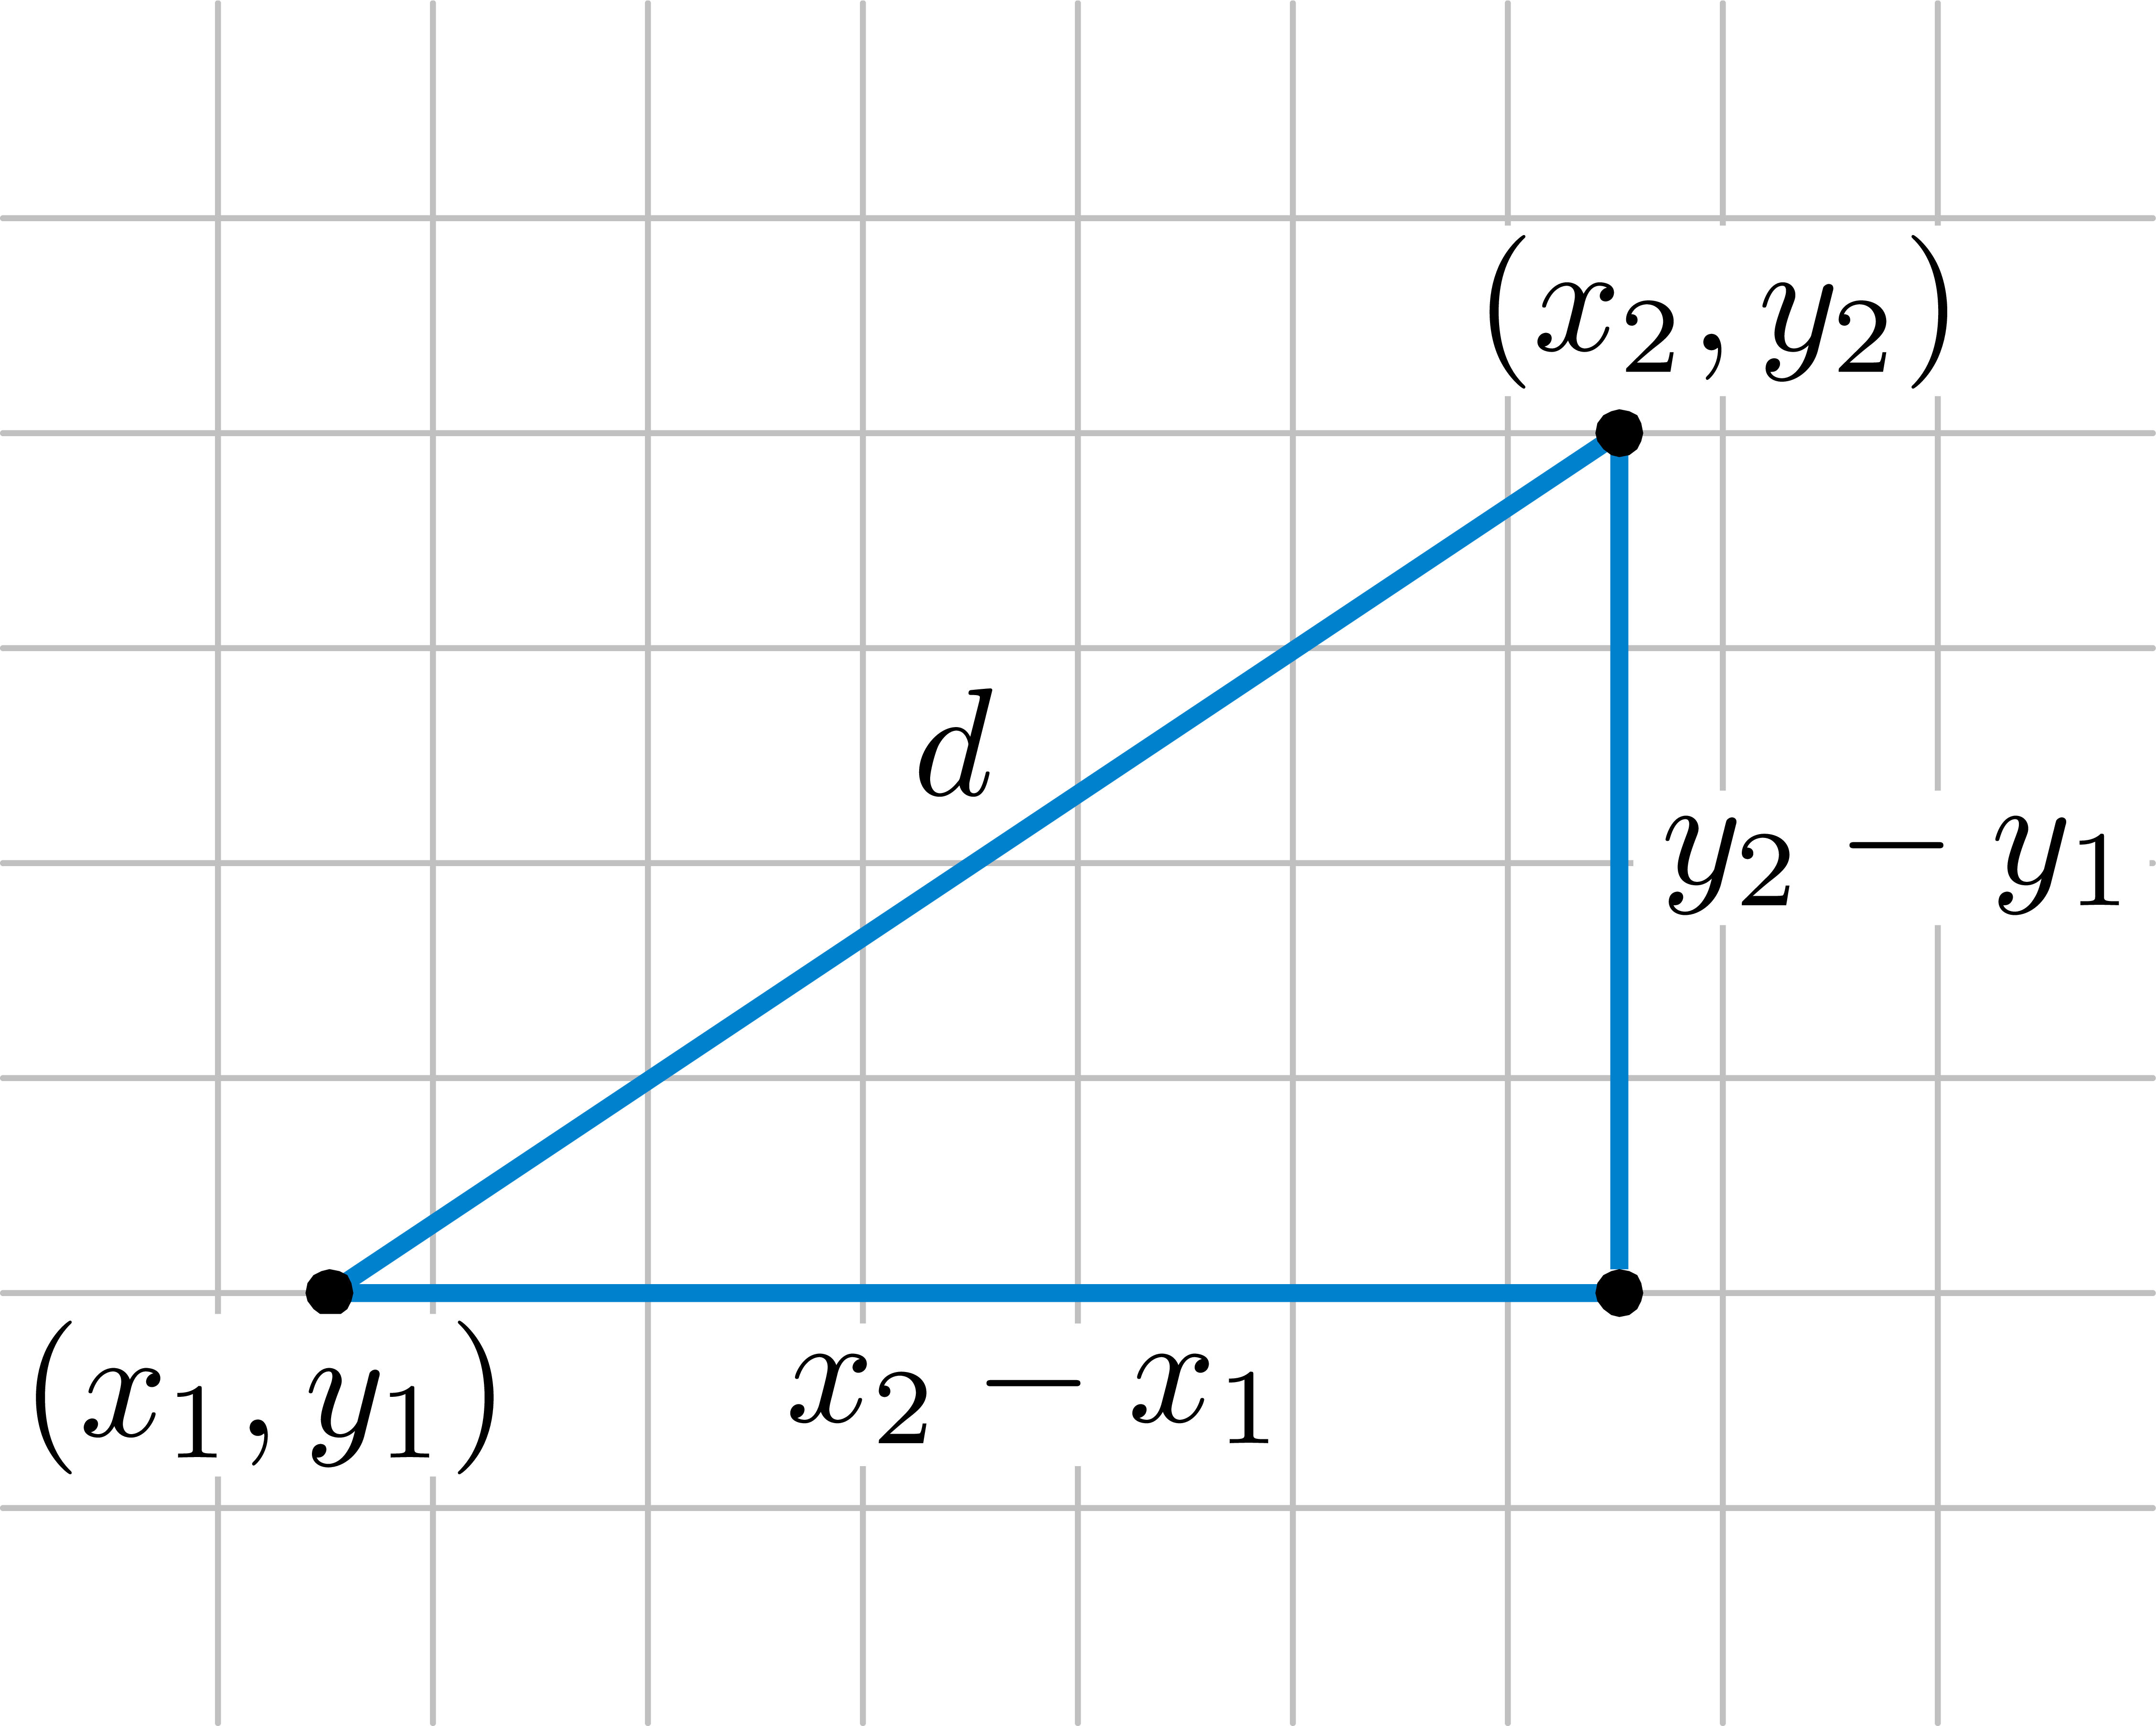
\includegraphics[scale=0.14]{Distance_Formula.jpg}
			\end{wrapfigure}
			Consider the following for $(x_1, y_1), (x_2, y_2)$.
			\begin{align}
				d^2 & = \lvert x_2 - x_1 \rvert ^2 + \lvert y_2 - y_1 \rvert ^2 \\
			      d & = \sqrt{\lvert x_2 - x_1 \rvert ^2 + \lvert y_2 - y_1 \rvert ^2} \\
			      	& = \sqrt{(x_2 - x_1)^2 + (y_2 - y_1)^2} \label{df}
			\end{align}
		
			\subsection{Example Problem}
				Find the distance between $(-2, 5)$ and $(4, -3)$ using the distance formula (\ref{df}).
				\begin{align*}
					d & = \sqrt{(4--2)^2 + (-3-5)^2} \\
					  & = \sqrt{36 + 64} \\
					  & = \sqrt{100} \\
					  & = 10
				\end{align*}
	
		\section{Verify right triangle}
			Given $a$, $b$, and $c$ prove that a right triangle can be created with those side lengths.\\
			If the largest value is not equal to the sum of the two smaller values a right triangle cannot be created
			
			\subsection{Example Problem}
				Prove that a triangle can(not) be created with side lengths $\sqrt{5}$, $\sqrt{45}$, and $\sqrt{50}$.\\
				$\sqrt{50}$ is the longest side length, so we have to see if it is the sum of the smaller sides.
				\begin{align*}
					\sqrt{50} &\stackrel{?}{=} \sqrt{5} + \sqrt{45} \\
					\sqrt{50} &= \sqrt{50}
				\end{align*}
		
		\section{Homework}
			\begin{figure} % TODO: Make this figure go in the correct spot
				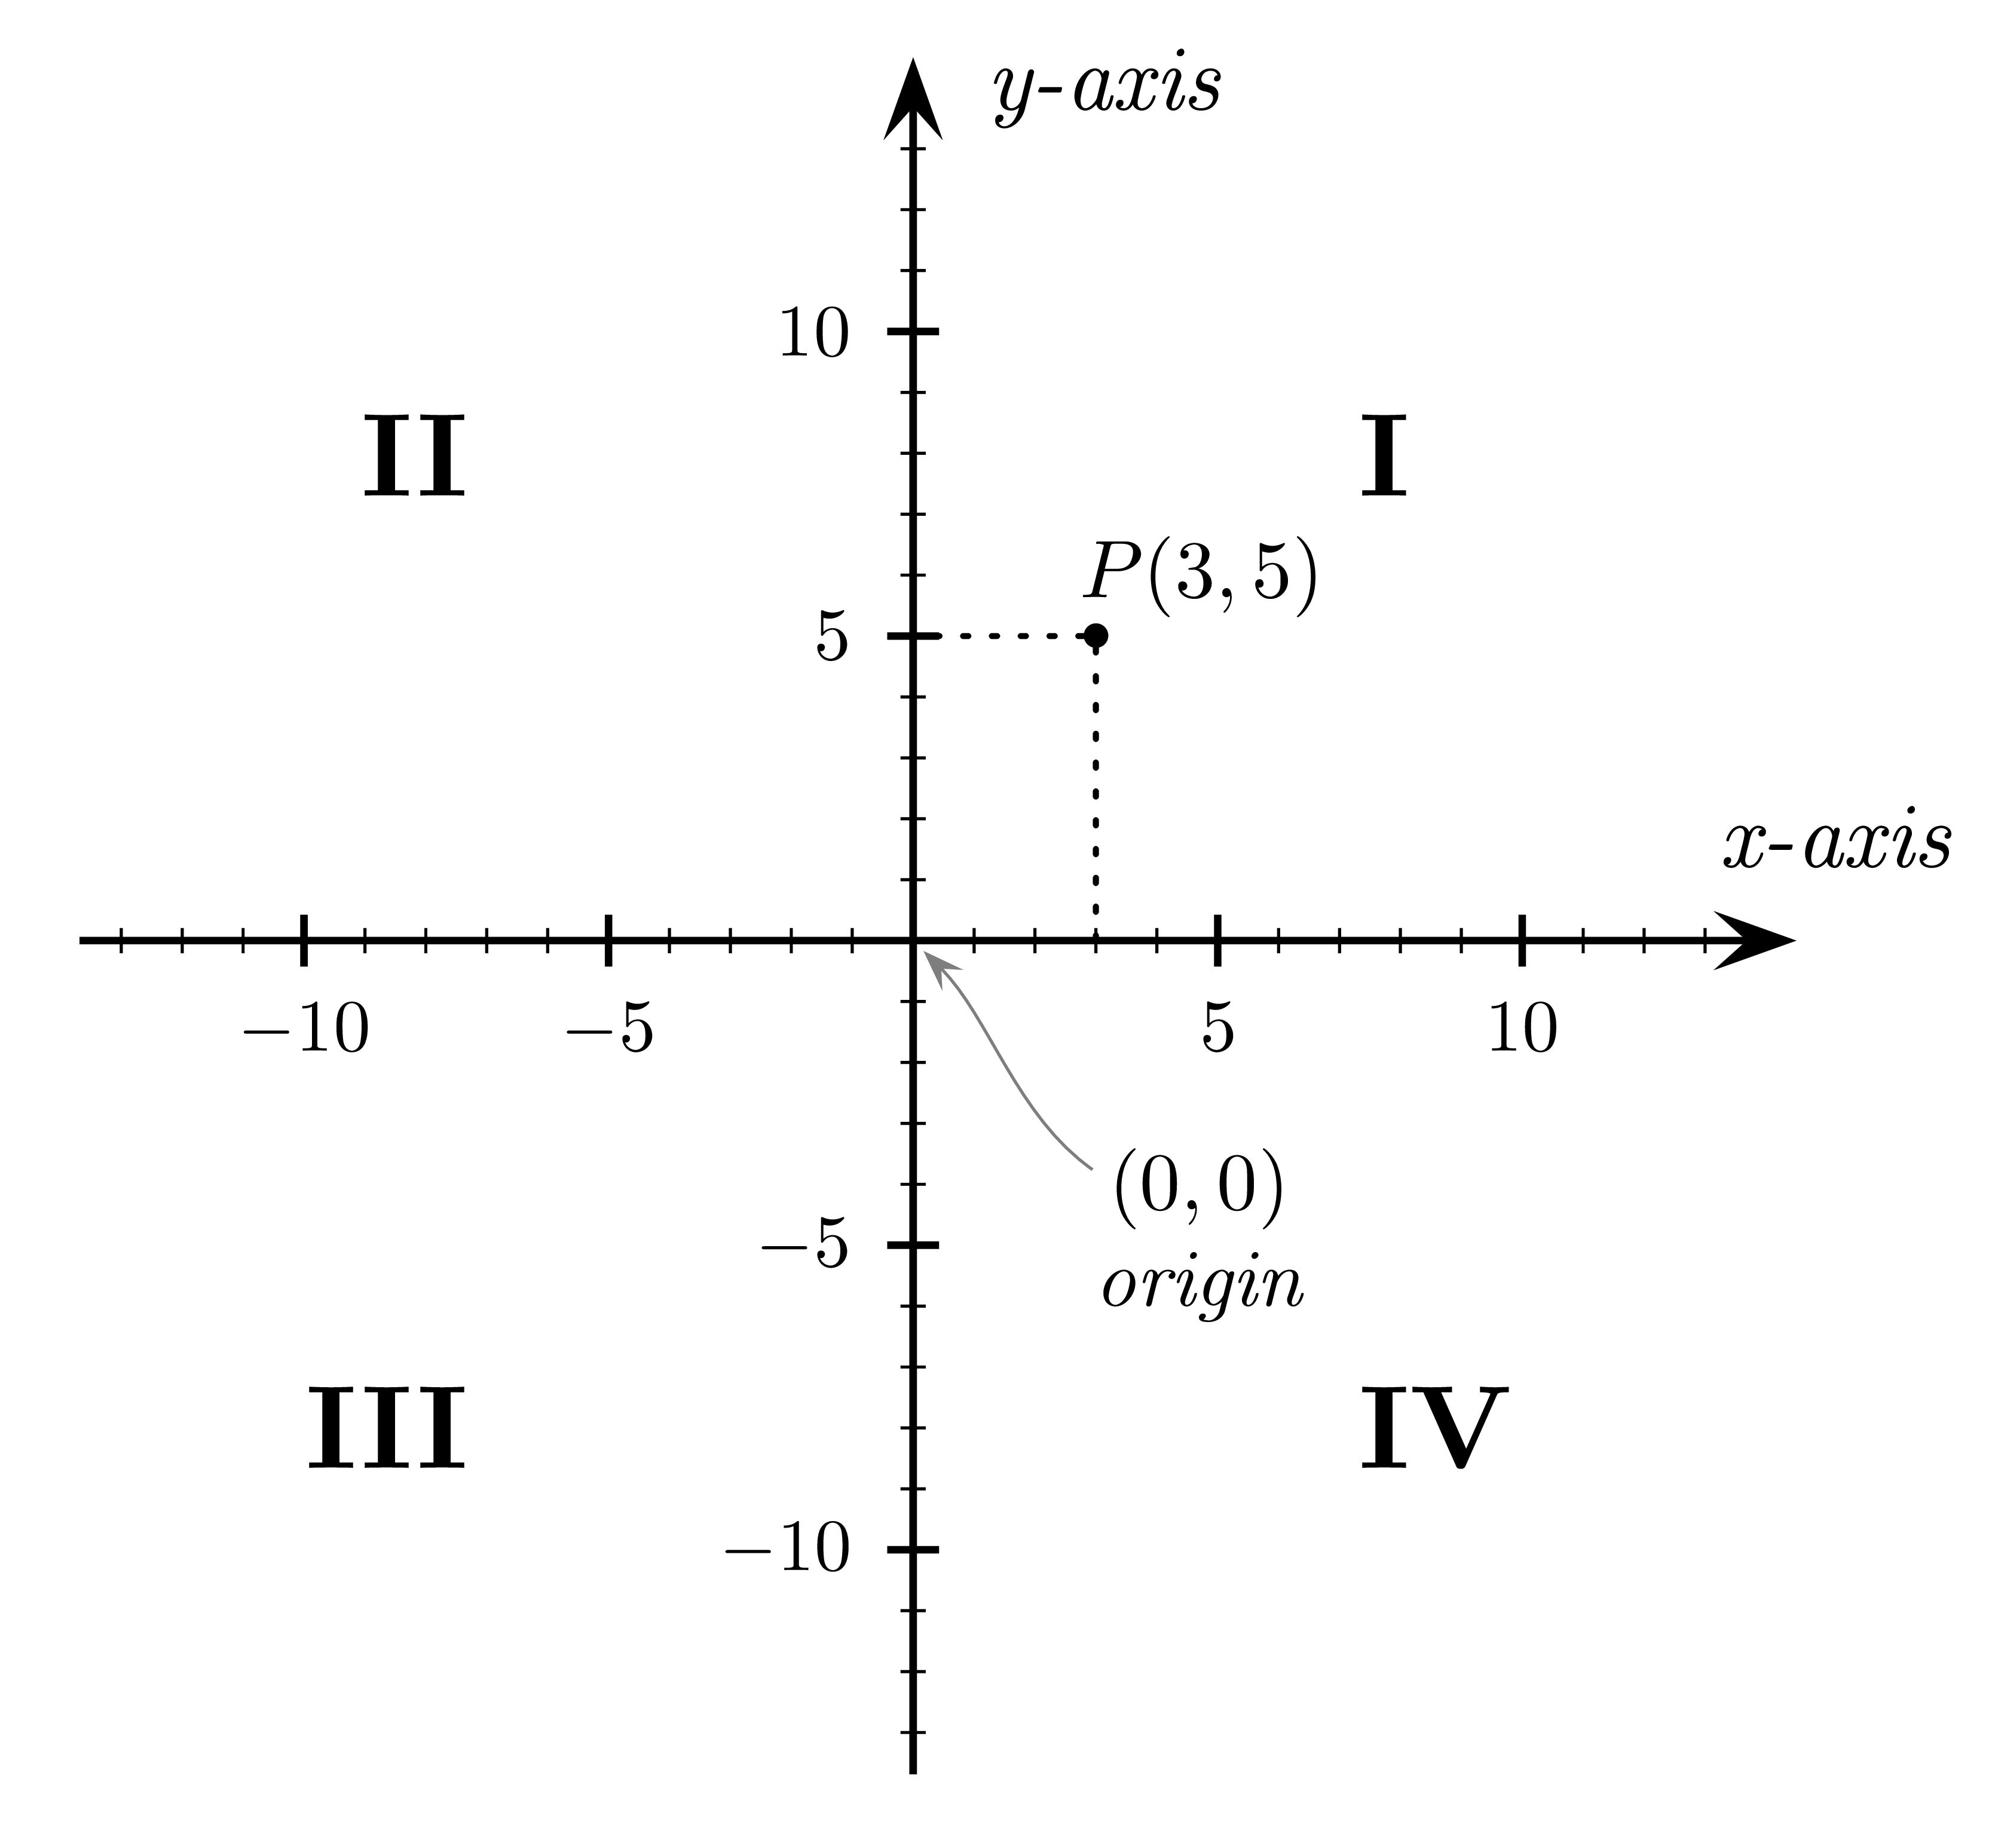
\includegraphics[scale=0.1]{Grid_Quads.jpg}
			\end{figure}
			\begin{enumerate}[widest={1}]
				\item[1] Determine the quadrant(s) in which $(x, y)$ could be located. (Select all that apply.)
				\begin{align*}
					x < 0 \text{ and } y > 0
				\end{align*}
				This pair could only be located in the 2nd quadrant.
				\item[2] Determine the quadrant(s) in which $(x, y)$ could be located. (Select all that apply.)
				\begin{align*}
					x < 0 \text{ and } y < 0
				\end{align*}
				This pair could only be located in the 3rd quadrant.
				\item[3] Determine the quadrant(s) in which $(x, y)$ could be located. (Select all that apply.)
				\begin{align*}
					x < 0 \text{ and } y = 6
				\end{align*}
				This pair could only be located in the 2nd quadrant.
				\item[4] Determine the quadrant(s) in which $(x, y)$ could be located. (Select all that apply.)
				\begin{align*}
					xy > 0
				\end{align*}
				This pair could be located in either the 1st or the 3rd quadrant.
				\item[6]
				\begin{enumerate}
					\item[(a)] Find the length of each side of the right triangle \\
					\begin{align*}
						& \text{distance between }(1, 2)\text{ and }(13, 2)&d_1 &= \sqrt{(1-13)^2+(2-2)^2} \\
						&&&= 12 \\
						& \text{distance between }(13, 2)\text{ and }(13, 11)&d_2 &= \sqrt{(13-13)^2+(2-11)^2} \\
						&&&= 9 \\
						& \text{distance between }(1, 2)\text{ and }(13, 11)&d_3 &= \sqrt{(1-13)^2+(11--13)^2} \\
						&&&= 15
					\end{align*}
					\item[(b)] Show that these lengths satisfy the Pythagorean Theorem.
					\begin{align*}
						d_1^2 &= 12^2 \\
						&= 144 \\
						d_2^2 &= 9^2 \\
						&= 81 \\
						d_1^2 + d_2^2 &= 255 = d_3^2
					\end{align*}
				\end{enumerate}
				\item[7] Consider the following. $(5, 3), (8, 3)$
				\begin{enumerate}
					\item[(a)] Plot the points
					\item[(b)] Find the distance between the points.
					\begin{align*}
						d &= \sqrt{(5-8)^2+(3-3)^2} \\
						  &= 3 \text{ units}
					\end{align*}
					\item[(c)] Find the midpoint of the line segment joining the points. \\
					\begin{align*}
						(x, y) = (\frac{a}{b}, \frac{c}{d})
					\end{align*}
				\end{enumerate}
			\end{enumerate}
		

\end{document}